In section~\ref{introOverview}, six core components of this project were identified. The first
three~-- ODE solving, rigid body dynamics and articulated bodies~-- were introduced in the last
chapter. In this chapter I give details of how the whole simulation was implemented in software,
and which challenges I faced along the way (section~\ref{implementation}). I then elaborate on
the three remaining components~-- collision detection (section~\ref{collisionDetection}), and
handling of colliding and resting contacts (section~\ref{collisionHandling}).


\section{Casting theory into code\label{implementation}}

My final implementation comprises 700 lines of \textsl{Octave} code (prototyping and numerical
tools) and 10500 lines of \textsl{Java} code for the main implementation (including 3500 lines
automatically generated by the XML data binding tool), plus a few fragments in other languages.

\subsection{The engineering process\label{engineering}}

The primary management challenge was to control the uncertainties caused by my lack of prior
knowledge of the algorithmic details required. The first four milestones, up to collision
detection, bore no major uncertainties, and could therefore be accomplished on schedule. I started
surveying the options for implementing articulated bodies during milestone~2; at this point I
realized that it was going to be much more challenging than expected, and that I would have to
adapt my strategy.

I decided to suspend coding after milestone~4 and to work on the theory until I was certain that
I understood it. If I tried to implement my ideas immediately, I believe the result would have
been chaotic and a waste of time. I set myself a new hierarchy of tasks arranged in a rectangular
grid. From left to right, the columns were the simulation components as listed in
section~\ref{introOverview} (except for item~4, which was already completed). From top to bottom,
the rows were labelled
\begin{enumerate}
\item search for literature relevant to the subject;
\item read and completely understand it;
\item if it is insufficient and no more literature can be found, work out a new algorithm for
    doing it;
\item argue or prove that the algorithm works correctly;
\item write down a good explanation of the algorithm, as if it were for another person to read, to
    ensure I fully understand it;
\item write a prototype in \textsl{Octave}.
\end{enumerate}

The idea of this grid is that each cell~-- one of these six tasks applied to one of the five
simulation components~-- depends on those above and to the left of it. Thus I could start in the
top left-hand corner and work towards the bottom right-hand corner; backtracking was possible when
I got stuck, but there was a clear objective and I could track progress. I decided that only
once I had covered the whole grid would I lay out and implement the \textsl{Java} program.
Completing the grid took me seven weeks, from mid-December until the end of January.

The \textsl{Java} implementation, testing and debugging were completed in the following seven
weeks, slightly less than the nine weeks originally allocated to this part of the project.
Including the seven additional weeks required to complete the ``theory grid'', the project was
now five weeks behind schedule.

Writing the dissertation, again a task with few uncertainties, took the allotted length of time.
With five weeks delay carried over and one week of holiday, the project finished six weeks behind
schedule. Given the early completion date (19~March) originally envisaged, this still
allowed me to submit well before the deadline.


\subsection{Application architecture\label{architecture}}

The \textsl{Java} implementation consists of five packages:

\begin{description}
\item[Scene.] Facilities to load a scene description from an XML input file, and data structures
    to represent it at run-time. This package is automatically generated by the data binding tool.
\item[Maths.] \sloppypar General-purpose implementations of vectors, matrices (including spar\-se
    matrices), quaternions, solver for ordinary differential equations (va\-ri\-able-step-size
    Runge-Kutta with Cash-Karp parameters~\cite{NRinC}), and a solver for systems of linear
    equations (biconjugate gradient method, also taken from~\cite{NRinC}).
\item[Geometry.] Handling of triangle meshes at run-time: deformation of articulated meshes,
    rendering of meshes using \textsl{Java3D}, collision detection. (Depends on Scene and Maths)
\item[Dynamics.] Implementations of a rigid body and all the different constraint types.
    Architecture for handling interactions between objects. Articulated body code combining
    rigid bodies and constraints, and implementation of the collision/contact handling algorithms.
    (Depends on Scene, Maths and Geometry)
\item[Main.] Main application class and test cases. (Depends on Scene and Dynamics)
\end{description}

The application follows a clean object-oriented design throughout. Some excerpts from its
class/interface hierarchy are shown in figure~\ref{classHierarchy}. This diagram indicates how
extensible the architecture is: any two \textsf{SimulationObject}s can interact, generating an
\textsf{Interaction} object~-- this could be anything from a repulsive Coulomb force to some
sort of sentient behaviour~-- without having to change any of the rest of the system.

\begin{figure}
\centerline{\scalebox{0.4}{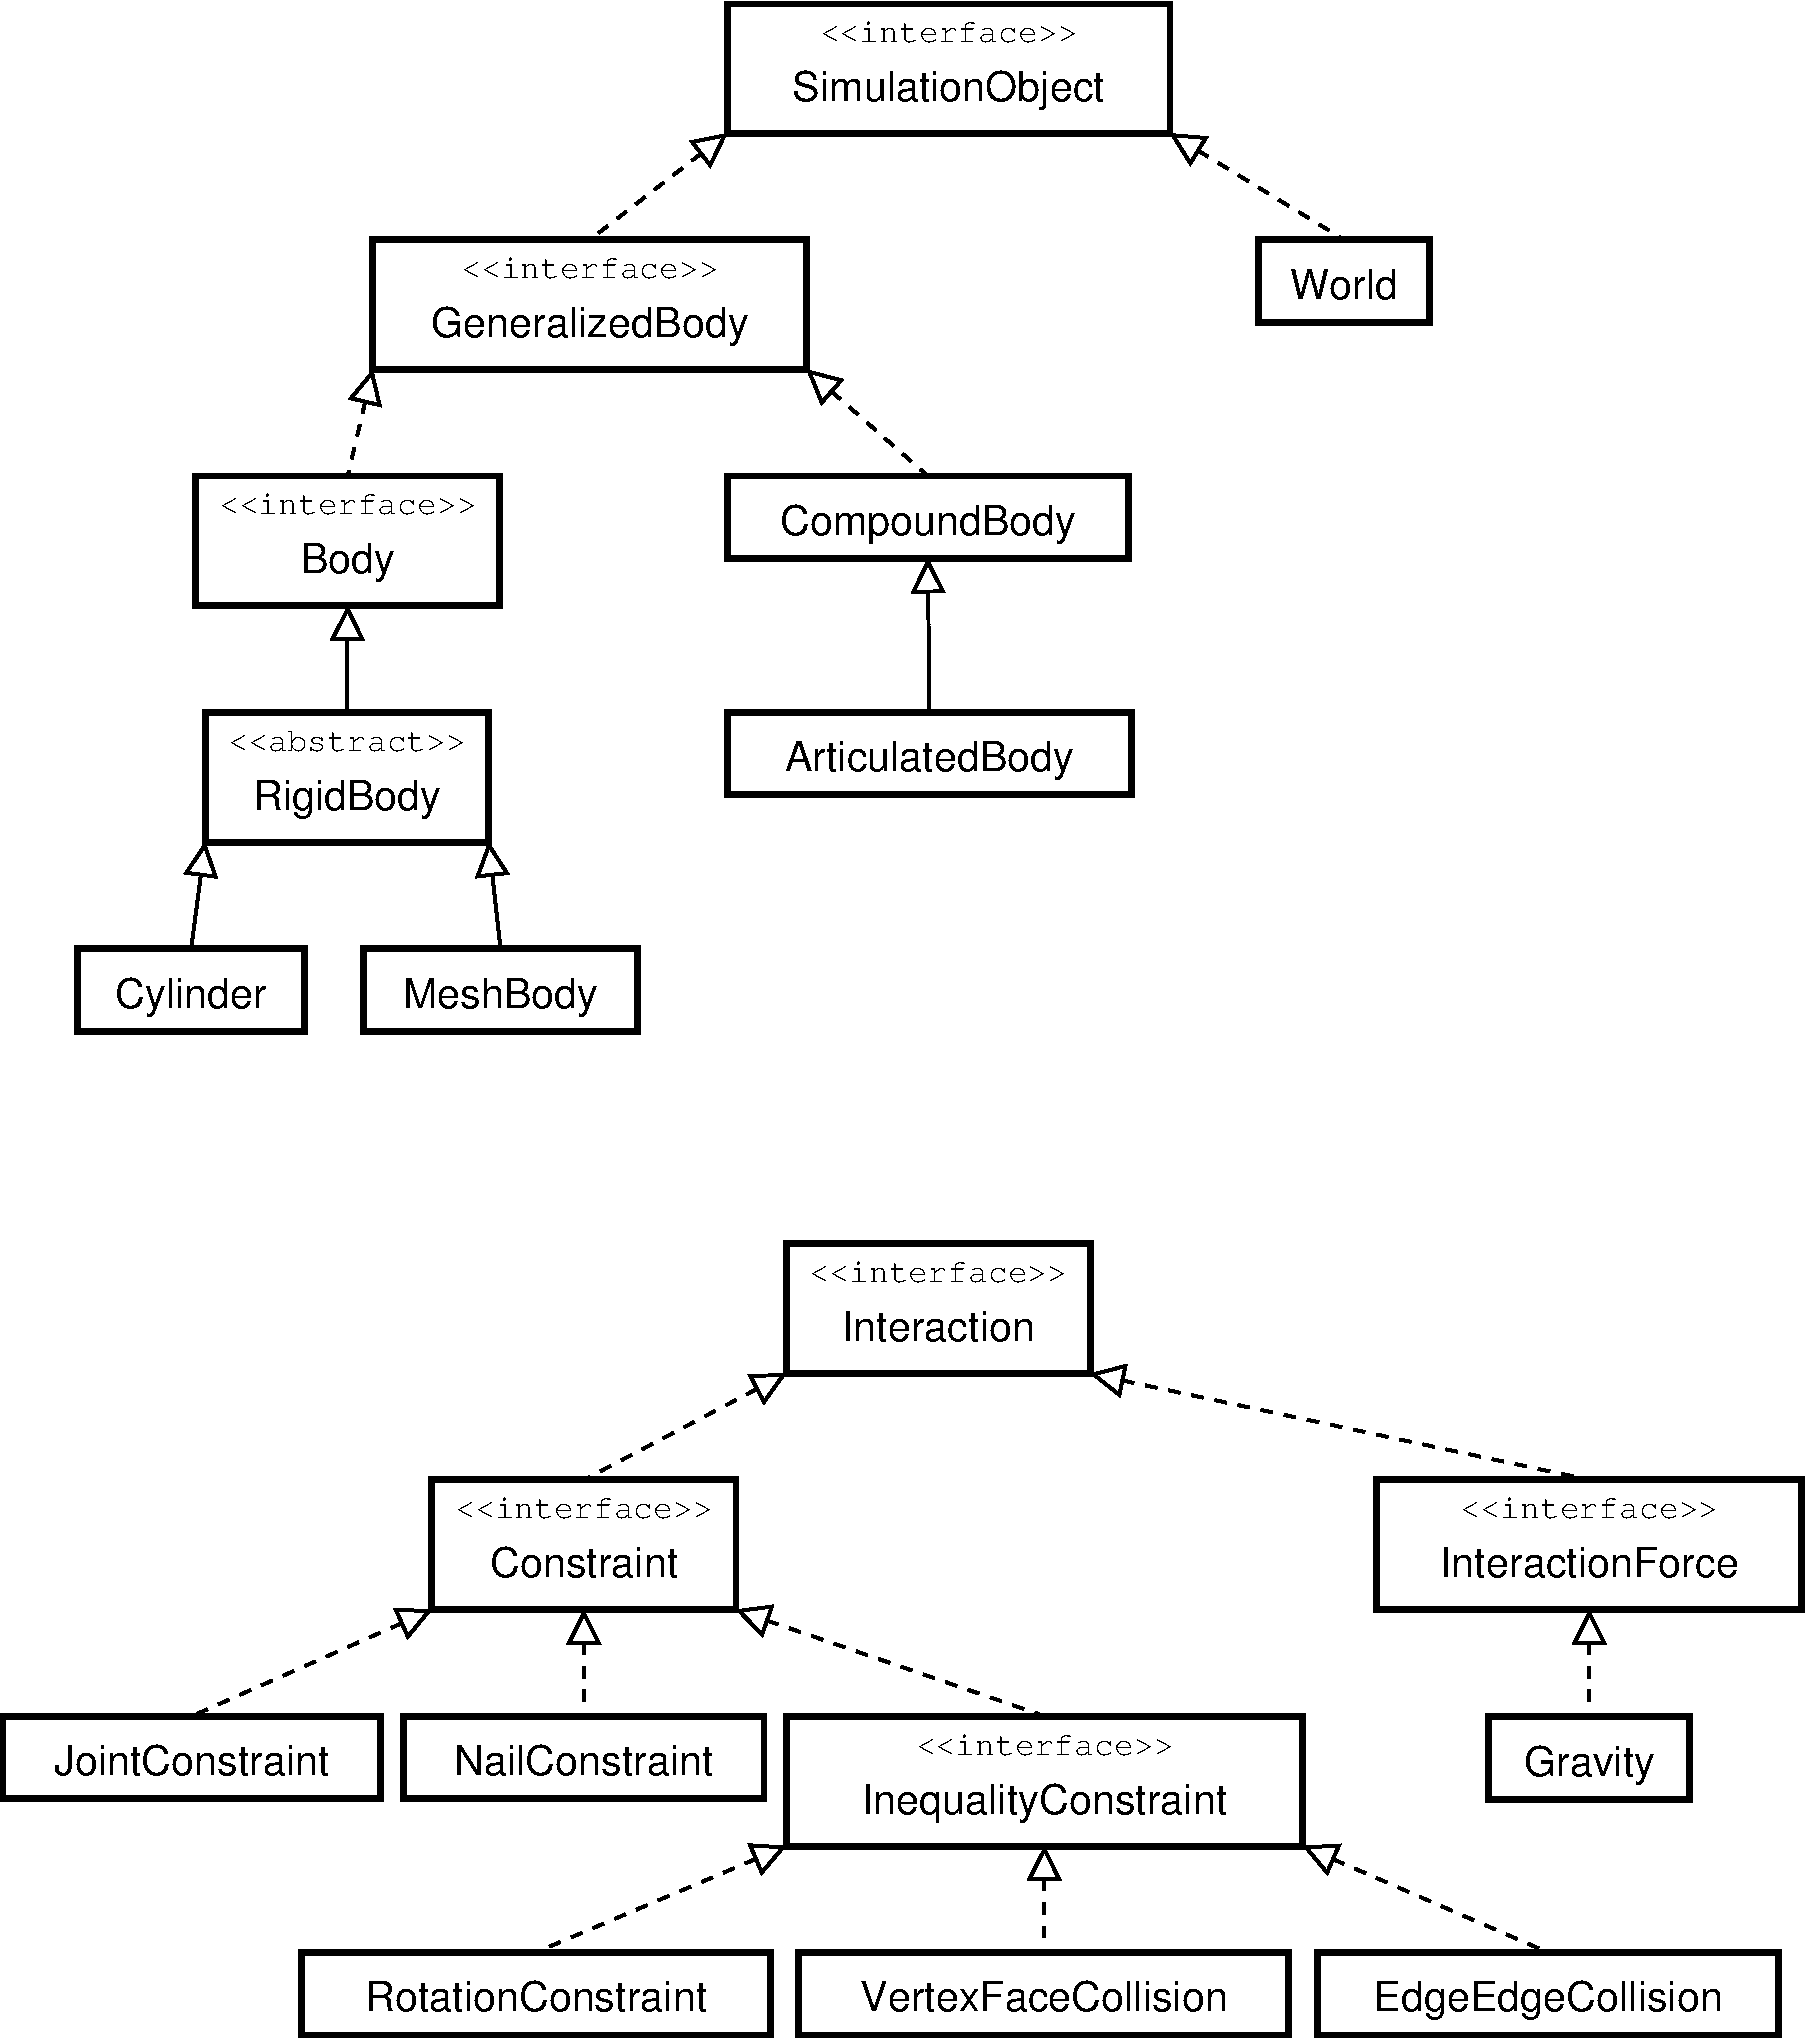
\includegraphics{figures/classes}}}
\caption{Two class inheritance hierarchies from the Dynamics package. Methods are omitted for
    better readability.\label{classHierarchy}}
\end{figure}

This design encapsulates algorithms in a way which is both clear and efficient. To give but two
examples:
\begin{itemize}
\item the ODE solver operates on the \textsf{Vector} interface. The \textsf{RigidBody}'s
    state vector implements the \textsf{add} method in such a way that quaternions are
    automatically normalized when appropriate. Thus the ODE solver needs to know nothing about
    quaternions, and a \textsf{RigidBody} object can be handled by any ODE solver.
\item the biconjugate gradient method for solving linear equations only multiplies \textsf{Matrix}
    objects with \textsf{Vector}s. This operation is implemented efficiently for sparse matrices,
    so the algorithm can run quickly even though it knows nothing about sparsity itself.
\end{itemize}


\subsection{Making it work\label{algorithmImplementation}}

A flow chart of the main simulation loop is given in figure~\ref{flowchart}. The main algorithmic
building blocks are indicated on the right margin. The order in which the steps is performed is
important, and it took me several attempts to get this right~-- despite careful thought
beforehand~-- because the bugs were quite subtle. The step size can be varied both by the ODE
solver error estimation and by the Newton-Raphson collision time search. This would not have
been possible with a library implementation of either algorithm.

\begin{figure}
\renewcommand{\baselinestretch}{1.25}\small\normalsize
\newcommand{\spx}{\vspace*{\baselineskip}\\}
\newcommand{\curly}[2]{\zerobox{b}{\mbox{$\left\}\:#1\begin{array}{l}#2\end{array}\right.$}}}
\begin{tabular}{|l|l|l|l|@{}l}
\multicolumn{5}{r}{explained in section $\downarrow$}\\\cline{1-4}
\multicolumn{4}{|l|}{Load scene and initial state from XML file}
&\curly{\ref{softwareTools}}{\spx}\hspace*{7mm}\\\cline{1-4}
\multicolumn{4}{|l|}{Compute initial set of interactions and constraints}&
\curly{\ref{meshIntersection}}{\spx}\\\cline{1-4}
\multicolumn{4}{|l|}{Choose initial time step length $h$}\\\cline{1-4}
\multicolumn{4}{|l|}{Repeat:}\\\cline{2-4}
    &\multicolumn{3}{|l|}{\texttt{Time step:}}\\\cline{2-4}
    &\multicolumn{3}{|l|}{For each time and state required by Runge-Kutta/Cash-Karp:}&
    \curly{\ref{solvingODEs}}{\spx}\\\cline{3-4}
        &&\multicolumn{2}{|l|}{Apply non-constraint forces (e.g.\ gravity)}\\\cline{3-4}
        &&\multicolumn{2}{|l|}{$\mbox{\textit{constraints}} = \mbox{\textit{equality constraints}}
        \cup \mbox{\textit{contact constraints}}$}\\\cline{3-4}
        &&\multicolumn{2}{|l|}{Repeat:}\\\cline{4-4}
            &&&Solve \textit{constraints} for Lagrange multipliers (equation~\ref{lagrangeEquation})\\\cline{4-4}
            &&&$\mbox{\textit{separating}} = \mbox{contact constraints with a component } \lambda_i < 0$&
            \curly{\ref{restingContact}}{\spx\spx\spx\spx\spx\spx\spx}\\\cline{4-4}
            &&&$\mbox{\textit{constraints}} = \mbox{\textit{constraints}} \;\backslash\;
            \mbox{\textit{separating}}$\\\cline{4-4}
        &&\multicolumn{2}{|l|}{Until $\mbox{\textit{separating}} = \{\}$}\\\cline{3-4}
        &&\multicolumn{2}{|l|}{Apply constraint forces $\m{J}^T\ve{\lambda}$ to bodies}\\\cline{3-4}
        &&\multicolumn{2}{|l|}{Compute derivative of state vector}&
        \curly{\ref{rigidBodyDynamics}}{\spx}\\\cline{2-4}
    &\multicolumn{3}{|l|}{Compute $O(h^4)$ and $O(h^5)$ approximations of new state vector}\\\cline{2-4}
    &\multicolumn{3}{|l|}{$\mbox{\textit{error}} = \mbox{difference between the approximations}$}\\\cline{2-4}
    &\multicolumn{3}{|l|}{If \textit{error} too large:}\\\cline{3-4}
        &&\multicolumn{2}{|l|}{Estimate new (smaller) value for $h$}&
        \curly{\ref{solvingODEs}}{\spx\spx\spx\spx\spx\spx\spx}\\\cline{3-4}
        &&\multicolumn{2}{|l|}{Goto \texttt{Time step}}\\\cline{2-4}
    &\multicolumn{3}{|l|}{Otherwise if error is small:}\\\cline{3-4}
        &&\multicolumn{2}{|l|}{Estimate new (larger) value for $h$ for the next time step}\\\cline{2-4}
    &\multicolumn{3}{|l|}{Compute interactions (e.g.\ collisions) in new state}&
    \curly{\ref{meshIntersection}}{\spx}\\\cline{2-4}
    &\multicolumn{3}{|l|}{If penetration has occurred:}\\\cline{3-4}
        &&\multicolumn{2}{|l|}{Estimate new (smaller) value for $h$ by Newton-Raphson}&
        \curly{\ref{findingContactTime}}{\spx\spx\spx}\\\cline{3-4}
        &&\multicolumn{2}{|l|}{Goto \texttt{Time step}}\\\cline{2-4}
    &\multicolumn{3}{|l|}{While there are colliding contacts:}\\\cline{3-4}
        &&\multicolumn{2}{|l|}{$\mbox{\textit{constraints}} = \mbox{\textit{equality constraints}}
        \cup \mbox{\textit{colliding contacts}}$}\\\cline{3-4}
        &&\multicolumn{2}{|l|}{Solve \textit{constraints} for Lagrange multipliers
        (equation~\ref{collisionLagrange})}&
        \curly{\ref{collidingContact}}{\spx\spx\spx\spx\spx}\\\cline{3-4}
        &&\multicolumn{2}{|l|}{Apply constraint impulses $\m{J}^T\ve{\lambda}$ to bodies}\\\cline{3-4}
        &&\multicolumn{2}{|l|}{Reclassify contact types according to new velocities}\\\cline{2-4}
    &\multicolumn{3}{|l|}{$\mbox{\textit{time}} = \mbox{\textit{time}} + h$}\\\cline{2-4}
    &\multicolumn{3}{|l|}{Output the simulation state for the current time}\\\cline{2-4}
\multicolumn{4}{|l|}{Until a predefined simulation time has been reached}\\\cline{1-4}
\end{tabular}
\caption{Overall (slightly simplified) structure of the simulation algorithm.\label{flowchart}}
\end{figure}

There was only one major design mistake which I had to correct during the debugging phase: I had
originally decided to store the current state of the simulation as values in each
\textsf{RigidBody} object. This caused errors when the simulation had to backtrack and retry a
step, because part of the body state had already been overwritten by the aborted step and could
not be regained without introducing tight coupling with the ODE solver. I changed the architecture
such that all time-varying state of a body is kept in a separate, immutable state vector, and all
operations require the current state as an argument, returning a new state. These side-effect-free
semantics made juggling different simulation states much easier, but the rewriting effort
to incorporate this architecture change took almost a week~-- it would have been no difficulty
if I had initially designed it this way.

I did not invest much effort in improving the run-time performance, but I did perform some
profiling which showed that a very large proportion of the time was being spent in the biconjugate
gradient solver for linear equations. I had originally implemented the \emph{preconditioned}
version of this algorithm described in~\cite{NRinC}, but noticed in the profiler that computing
the preconditioner matrix was more expensive than its benefit. Removing the preconditioning
immediately increased the execution speed of the whole simulation by a factor of 18.


\subsection{Extensions\label{extensions}}

Being significantly behind schedule towards the end of the project, I decided not to add many
optional features~-- I merely wrote a short but exceedingly useful script to import completed
simulations into \textsl{Blender}, in order to create raytraced video files.
